\documentclass[10pt,english]{article}
\usepackage[utf8]{inputenc}
\markright{Weedop et al.\hfill The Effect of Phylogenetic Uncertainty and Imputation on EDGE Scores\hfill}
\usepackage{geometry}
\usepackage[labelfont=bf]{caption}
\usepackage{makecell}
\geometry{verbose,letterpaper,tmargin=2.54cm,bmargin=2.54cm,lmargin=2.54cm,rmargin=2.54cm}
%\geometry{verbose,letterpaper,tmargin=.1cm,bmargin=.1cm,lmargin=.1cm,rmargin=.1cm}
\usepackage{graphicx}
\DeclareGraphicsExtensions{.pdf,.png,.jpg}
\usepackage{amssymb,amsmath}
\usepackage{epstopdf}
\usepackage{tocbibind}
\usepackage[toc,page]{appendix}
\usepackage{supertabular}
\DeclareGraphicsRule{.tif}{png}{.png}{`convert #1 `dirname #1`/`basename #1 .tif`.png}
\usepackage{url}
\usepackage{subcaption}
\usepackage{caption}
\usepackage[super]{nth}
\usepackage{lineno} \linenumbers
\usepackage[doublespacing]{setspace}
\usepackage[parfill]{parskip}
\setlength{\parindent}{0pt}
\usepackage{csquotes}
\usepackage[backend=biber, 
            natbib=true,
            style=authoryear, 
            citetracker=true, 
            maxcitenames=2, 
            uniquelist=false, 
            uniquename=false]{biblatex}

\AtEveryCitekey{\ifciteseen{}{\defcounter{maxnames}{3}}}
\renewbibmacro{in:}{}
\DeclareFieldFormat[article, inbook, incollection, inproceedings, misc, thesis, unpublished]{title}{#1}
\DeclareFieldFormat[article, inbook, incollection, inproceedings, misc, thesis, unpublished]{pages}{#1}
\addbibresource{edge_sims.bib}

\DeclareFieldFormat[article]{volume}{#1}
\setlength{\bibhang}{0pt}

\usepackage{changes}
\setdeletedmarkup{\textcolor{red}{\sout{#1}}}

\begin{document}
\setlength{\parindent}{0pt}
\section*{Title page}

\textbf{Article title}: The Effect of Phylogenetic Uncertainty and Imputation on EDGE Scores

\textbf{Running Head}: Effects of Phylogenetic Uncertainty and Imputation on EDGE

\textbf{Authors:} K.\ Bodie Weedop$^{1*}$, Arne \O. Mooers$^2$, Caroline M.\ Tucker$^3$, and William D.\ Pearse$^{1}$\

$^1$ Department of Biology \& Ecology Center, Utah State University,
5305 Old Main Hill, Logan UT, 84322

$^2$ Department of Biological Sciences, Simon Fraser University, Burnaby,
British Columbia, Canada

$^3$ Department of Biology, University of North Carolina–Chapel Hill

$^*$To whom correspondence should be addressed: K.\ Bodie Weedop (\url{kbweedop@gmail.com})

\clearpage
\section*{Abstract}

Faced with the challenge of saving as much diversity as possible given financial
and time constraints, conservation biologists are increasingly prioritizing
species on the basis of their overall contribution to evolutionary diversity.
Metrics such as EDGE (Evolutionary Distinct and Globally Endangered) have been
used to set such evolutionarily-based conservation priorities for a number of
taxa, such as mammals, birds, corals, amphibians, and sharks. Each application
of EDGE has required some form of correction to account for species whose
position within the tree of life are unknown. Perhaps the most advanced of these
corrections is phylogenetic imputation, but to date there has been no systematic
assessment of both the sensitivity of EDGE scores to a phylogeny missing
species, and the impact of using imputation to correct for species missing from
the tree. Here we perform such an assessment, by simulating phylogenies,
removing some species to make the phylogeny incomplete, imputating the position
of those species, and measuring (1) how robust ED scores are for the species
that are not removed and (2) how accurate the ED scores are for those removed
and then imputed. We find that the EDGE ranking for species on a tree is
remarkably robust to missing species from that tree, but that phylogenetic
imputation for missing species, while unbiased, does not accurately reconstruct
species’ evolutionary distinctiveness. On the basis of these results, we provide
clear guidance for EDGE scoring in the face of phylogenetic uncertainty.

\textbf{Keywords}: conservation prioritization, evolutionary distinctiveness, 
EDGE, phylogenetic imputation

\clearpage
\section*{Introduction}

Evidence from the fossil record and present-day studies argue we are in the
midst of, or entering, a sixth mass extinction \autocite{Barnosky2011,
Ceballos2015}, such that more populations than ever are declining and species
face heightened danger of extinction \autocite{Wake2008, Thomas2004}. Habitat
destruction \autocite{Brooks2002}, invasive species \autocite{Molnar2008},
climate change \autocite{Pounds2006}, and disease \autocite{Lips2006} are some
of the leading causes of species declines globally. Conservation biologists seek
to reduce these detrimental effects on species populations, but in reality they
have limited resources with which to do so. This challenge, termed the “Noah's
Ark problem” \autocite{Weitzman1998}, has driven conservation biologists to
identify different ways by which to prioritize, or triage, their resource
allocation \autocite{Bottrill2008}.

Conservation triage, like all sound decision-making, requires a method to
quantify the relative urgency or importance for conservation among a set of
options. This allows scientists and policy-makers to use data to quantify need
and inform conservation decision-making and management activities. One triage
strategy uses the EDGE metric to identify and prioritize species that are
Evolutionarily Distinct and Globally Endangered \autocite{Isaac2007}.
Evolutionary Distinctiveness (ED) measures the relative contributions made by
each species within a particular clade to phylogenetic diversity, assigning each
branch length equally to all the subtending species \autocite{Redding2003,
Isaac2007}. Global Endangerment (GE), assigns numerical values to each of the
International Union for Conservation of Nature (IUCN) Red List Categories. As
species become increasingly threatened and are placed into categories of
increasing concern (\emph{e.g.} from Vulnerable to Endangered), the GE numerical
value increases. A species’ EDGE score is an aggregate value intended to equally
reflect a species’ evolutionary distinctiveness and conservation status
\autocite[even if it does not always in practice; see][]{Pearse2015}.

Usage of the EDGE metric has expanded greatly. First used to prioritize global
mammals \autocite{Isaac2007}, EDGE scores are now available for a variety of
taxonomic groups, including amphibians \autocite{Isaac2012}, birds
\autocite{Jetz2014}, corals \autocite{Curnick2015}, squamate reptiles
\autocite{Tonini2016}, sharks \autocite{Stein2018}, and all tetrapods
\autocite{Gumbs2018}. Related metrics are also now available, each subtly
emphasizing different things, such as the expected contribution of each species
to future phylogenetic diversity \autocite[HEDGE,
I-HEDGE;][]{Steel2007,Jensen2016} and our uncertainty over a species' future
\autocite[EDAM;][]{Pearse2015} The development and expansion of EDGE-like
metrics mirrors progress in other areas of conservation biology, and the
likelihood of success in conservation \autocite{Wilson2007, Mcbride2007}, the
relative cost of certain interventions \autocite{Naidoo2006}, and
complementarity of interventions \autocite{Pressey1993, Myers2000} can now be
considered in its calculation. The EDGE index was developed explicitly with the
intention of informing conservation triage, and is now the basis of the global
EDGE of Existence Program (http://www.edgeofexistence.org/). The successful
application of EDGE highlights the potential for phylogenetic conservation
prioritization metrics to provide actionable insights while quantitatively
measuring the evolutionary history a species represents. Nonetheless, almost
every application of an EDGE-type approach must address uncertainty resulting
from missing data. Addressing, and hopefully improving, our ability to
handle uncertainty should be a continual effort to increase the support for such
approaches. \added{However, in an effort to dilineate between science and policy, it is
important to note that the implications of missing data on policy making will
vary depending upon the demands and goals of a particular person or
organization.}

Missing data can affect EDGE scores in several ways. First, the IUCN identifies
some species as Data Deficient \autocite{Iucn2001, Iucn2008}, which affects the
GE component of a species' EDGE score. Fortunately, the IUCN provides guidance
for using any available contextual data to assign some threat status to such
species. A number of studies illustrate how to assign threat categories to Data
Deficient species, which in turn should reduce the uncertainty in GE
\autocite{Good2006, Butchart2010, Morais2013, Dulvy2014}. The issue of missing
phylogenetic data is arguably more complicated because not only does the focal
species have no ED score, but its absence from the phylogeny may affect the ED
scores of related species. Species of conservation concern are almost by
definition rare, and frequently lack sufficient DNA (or even morphological) data
to be placed with certainty on a phylogeny. In most cases, taxonomic information
rather than sequence data alone has been used to place species in the tree of
life when constructing EDGE lists \autocite[see][]{Isaac2007, Collen2011,
Isaac2012, Jetz2014, Curnick2015, Stein2018, Gumbs2018, Forest2018}. Yet, to our
knowledge, there has been no systematic study of the effect of imputation on
species’ EDGE scores, despite this practice having received attention in other
areas of comparative biology \autocite{Kuhn2011, Thomas2013, Rabosky2015}. Thus
we do not know how accurate EDGE scores are when species are missing, or when
species are added to phylogenies by imputation, nor do we know how accurate EDGE
scores for imputed species might be. As interest in using EDGE-type measures
and phylogenies for conservation triage grows, the need for consensus on how to
resolve cases of phylogenetic uncertainty becomes increasingly urgent. 

Here we attempt to quantify the effect of one sort of phylogenetic
uncertainty---the effect of missing species on EDGE rankings---and assess the
degree to which subsequent imputation affects the accuracy of EDGE scores. We do
so by simulating phylogenies and then removing species either at random, or with
bias, across those phylogenies. By contrasting the ED scores of the species
before and after the loss of other species from the phylogenies, we measure the
impact of missing species on ED scores. We then assess the extent to which
phylogenetic imputation can accurately estimate the EDGE scores of missing
species in simulated data. We also examine the extent to which such imputation
affects the scores of species for which we have data. In doing so, we hope to
provide clear guidance as to the applicability of phylogenetic imputation as a
solution for species missing phylogenetic data. From our results, we argue that
species' ED values are remarkably robust to missing species, and that
phylogenetic imputation does not reliably reconstruct the true ranking of those
missing species.

\section*{Methods}

We use a simulation approach to test the effect of having missing species
on a phylogeny (through species removal from simulated phylogenies) and then
imputing species for species’ ED (Evolutionary Distinctiveness) scores. We focus
exclusively on the ED-component of the EDGE metric, since uncertainty in species
GE scores has already been addressed by the IUCN’s proposal to assign Data
Deficient species scores \autocite{Iucn2001, Iucn2008}. Because EDGE is the
product of both ED and GE components, even perfectly accurate GE values could be
associated with imperfect EDGE scores if the ED scores were inaccurate.

All trees (both starting and imputed) were simulated under a pure-birth Yule
model using 'gieger::sim.bdtree' \autocite[setting parameters \texttt{b=1} and
\texttt{d=0};][]{Pennell2014}. This model was chosen because it is the simplest
model possible: speciation rates are constant across the entire tree of life and
there is no extinction. We suggest that imputation under a simple model that is
identical to that used to simulate the data is a low, and fair, benchmark for a
method to meet. However, we acknowledge that more complex and/or biologically
realistic models of diversification could potentially improve the performance of
imputation. We used 'caper::ed.calc' to calculate ED values \autocite{Orme2013}.
All simulations and analyses were performed using R \autocite[version
3.4.0;][]{R2017}. We performed 100 replicate simulations of each parameter
combination. All our analysis code is available online
(\url{https://github.com/bweedop/edgeSims}).

\subsection*{The impact of missing species on EDGE scores}
Our first set of simulations assess the impact of missing species data on the ED
scores of remaining species, considering data missing either in a random or
phylogenetically-biased fashion. We simulated phylogenies of different sizes
(number of species: 64, 128, 256, ..., 2048, 4096) and then removed constant
fractions of tips from the tree (0\%, 1\%, 2\%, ..., 19\%, ..., 99\%). To
simulate species missing at random throughout the phylogeny, we used 'sample()'
to select the relevant fraction of species (rounded to the nearest whole number)
without replacement. To remove species in a phylogenetically-biased manner, we
used \textcite{Felsenstein2005}'s threshold model. We simulated a trait under a
constant rate Brownian-motion model ($\sigma$=0.5, starting root value = 1)
\autocite[using 'geiger::sim.char'][]{Pennell2014}. Species were then removed
from the tree if their simulated trait was in the upper quantile matching the
fraction of species to be removed. For example, if 10\% of species were to be
removed from the tree, the species with the highest 10\% of values would be
removed. This results in closely related species being removed more often than
expected by chance.

To quantify the effect of these manipulations, we calculated the ED values of
species that are not removed from a tree both before and after removal. We then
correlated these ED scores: if missing species do not affect ED values of the
remaining species, we would expect a strong, positive correlation between the ED
scores of the remaining species calculated before and after species were removed
from the phylogeny. We emphasize that species removed from the phylogeny are
omitted from this comparison. We outline our approach in figure
\ref{missingSpecies}.

\subsection*{The impact of phylogenetic imputation on EDGE scores}
Our second set of simulations tested the impact of imputation on ED scores
within an imputed clade. We used relatively small clades (5, 6, 7, ..., 30, 31,
32 species) from phylogenies of different sizes [128 ($2^7$), 147 ($2^{7.2}$,
168 ($2^{7.4}$), ... , 776 ($2^{9.6}$), 891 ($2^{9.8}$), 1024 ($2^{10}$)
species). We first randomly selected a clade to be removed from the ‘true' tree
and then simulated a new phylogeny of the same size as the removed clade. This
newly simulated clade was generated under the same pure-birth model as the
original phylogeny. We then placed the newly simulated clade in the full
phylogeny, in the same location as the removed clade. If a newly simulated clade
was so old that it was not possible to graft it into place, we discarded that
clade and simulated another. In an empirical study the model of evolution under
which the phylogeny had evolved would have to be estimated, which is an
additional source of error not considered here. We simulated each combination of
clade and total phylogeny sizes 100 times when using a pure-birth Yule
model and 5 times when simulating under models with past extinction. An
overview of our approach is given in figure \ref{imputeConcept}. 

To assess whether clades, once imputed, had similar ED scores to their true
values, we correlated the imputed ED scores with the true ED scores. We also
calculated the sum of the absolute change in ranked ED for all species, which is
particularly relevant for EDGE-listing as conservation actions are often focused
around the top 100, 200, etc., species. Moreover, the correlation of imputed and
real scores are bounded by the depth of the imputed clade, and therefore a high
correlation could still produce inaccurate imputed scores, and a low correlation
could still not be important (\emph{e.g.} they could be anticorrelated but still
differ in rank by a max of the size of the subclade). We modeled both of these
metrics (the change in ranking and the correlation) as a function of a number of
potential explanatory variables. Specifically, we included in our models: the
estimated speciation rate of the original phylogeny \autocite[using
`ape::yule';][]{Paradis2004}, the sum of all phylogenetic branch-lengths
in the original phylogeny \autocite[Faith's PD;][]{Faith1992}, the sum of all
phylogenetic branch-lengths in the original focal clade \autocite[Faith's
PD;][]{Faith1992}, the value of $\gamma$ in the original phylogeny
\autocite[using `phytools::gammatest';][]{Pybus2000, Revell2012},
Colless' index of the original phylogeny \autocite[using
`apTreeshape::as.treeshape';][]{Colless1982, Bortolussi2009}, the
kurtosis of species' ED values in the original phylogeny \autocite[using
`moments::kurtosis';][]{Komsta2015}, the skew of species' ED values in
the original phylogeny \autocite[using `moments::skew';][]{Komsta2015},
the total number of species in the original phylogeny, the total number of
species within the imputed clade, and the depth (age) of the imputed clade in
the phylogeny. Although the expectations of many of these explanatory variables
are known for Yule trees, in each simulation they are expected to vary somewhat
by chance.

Recently, there has been interest in assigning missing species the mean ED score
of the most exclusive clade which contain the species
\autocite[see][]{Gumbs2018}. To test the efficacy of such methods, we assigned
the average ED of the selected clade to each of its' species and calculated (as
above) the mean change in absolute ranking under this scheme. Note that we could
not correlate ED scores (as we do above), since such a correlation would require
variation in species' scores and under this approach a single score (the mean
ED) is assigned to all imputed species.

\added{We present, in the supplementary materials, two additional sets of analyses
intended to examine the impact that past extinction rates may have played on our
analyses. These simulations incorporate conditions of past extinction at low and
high rates using `gieger::sim.bdtree' \autocite[setting parameters for low
extinction at \texttt{b=1} and \texttt{d=0.5} and high extinction \texttt{b=1}
and \texttt{d=0.95};][]{Pennell2014}. These models represent large departures
from our main simulations (which have \texttt{b=1} and \texttt{d=0}), and so we
performed only 5 replicates per set of parameter combinations as our only aim
was to detect any major differences in our results stemming from these changes.
Otherwise, these simulations were identical to those we present in the main text.}


\section*{Results}
We asked how robust ED scores were for species with known positions on the
phylogeny, when other species were missing from the phylogeny. In fact, when
there were increasing numbers of missing species, ED scores for the remaining
species’ became less accurate (table 1; figure \ref{randomVsClustered}). When
species were missing from the tree in a phylogenetically-based fashion, ED
values were less robust as compared to when species are randomly missing from
the tree. However, the effect of missing species is not necessarily severe; even
if 20\% of species are missing from the tree, the average correlation
coefficient between true and estimated ED scores for the remaining species is
0.88 and 0.94 for phylogenetically-biased and random missing species,
respectively.

We also considered the impact of imputation on the accuracy of ED scores for
imputated species. When clades were imputed on the tree, we found a weak (if
any) average positive correlation between the imputed ED and true ED values for
species within the imputed clades (overall mean correlation of $0.197$ in a
statistical model with an $r^2$ of $0.5\%$; figure \ref{imputationTrend}, table
2). We also found no explanatory variables that explained significant variation
in this relationship (table 2; see Appendix S1 in Supporting Information).
However, we did find evidence that, when imputing larger clades, the variation
in the correlation between true and imputed ED scores decreases, although we
emphasise the effect is weak (see table 2). When considering rankings rather
than raw scores, we found that imputation can introduce sizable error into the
estimation of species' ED values (figure \ref{rankingError} and table
\ref{impute_rank}). This ranking error increased with the size of the imputed
clade and phylogeny (table \ref{impute_rank}), and can affect ranking error
within the top 100 and 250 species (see Appendix S2 in Supporting Information).
To give an example of the magnitude of the effect, within a phylogeny of 1024
species, the members of an imputed clade of 30 species are, on average, $\pm$
315 rankings from their true rankings. We found similar effects in ranking error
when using the average ED value of clade for a missing species (see Appendix S3
in Supporting Information). \added{As we show in the supplementary materials, the
simulation (and subsequent imputation) of phylogenies under models incorporating
extinction rates (\emph{i.e.}, not Yule models) had qualitatively identical
results. We do not, therefore, discuss them in detail here.}

\section*{Discussion}
Phylogenies are playing an increasing role in conservation prioritization,
decision-making, and policy \autocite{Vezquez1998, Veron2017}. A major obstacle
to a more widespread adoption of phylogenetic prioritization methods such as
EDGE is phylogenetic uncertainty \autocite{Collen2015}. There is a tension
between a purported need to make decisions to preserve biodiversity---including
evolutionary history---now, and the reality that we rarely have complete
information about the phylogenetic placement of many species of conservation
concern \autocite{Isaac2018}. The intention of our study is to
provide concrete information about the impact of one source of phylogenetic
uncertainty - missing species - on conservation prioritization. To address this
uncertainty, we addressed two key issues: (1) the extent to which species that
are missing from the tree of life impact the ED scores of species for which we
do have data, and (2) the extent to which phylogenetic imputation can accurately
estimate ED scores for taxa with no phylogenetic data. First, we found that
missing species had a surprisingly small impact on the ED scores of other
species, particularly if species are missing at random from the tree of life.
Second, we found that phylogenetic imputation generally fails to accurately
reconstruct species' ED scores and rankings.

\added{In this study, we have examined imputation under three separate models of
diversification: pure-birth Yule models (presented in the main text), and models
with relatively high and low rates of extinction (both in the Supporting
Information).} We acknowledge that lineages evolve in more complex
ways, although we suggest that focusing on these fundamental models of
diversification makes our results more broadly applicable. We suggest that a
method should perform well under basic conditions, and as such these results
form an appropriate benchmark, particularly given we can see no reason to
suppose that more complex models should increase model performance. Further, we
focus here solely on the results from a single imputation in each simulation,
despite, empirically, biologists reporting average ED scores calculated across
pseudo-posterior distributions of many imputed phylogenies \autocite{Kuhn2011}.
Thus our results show that the variation within these pseudo-posterior
distributions is likely very large. It is well-known that such imputation
methods are not biased \autocite[indeed, this was originally shown
by][]{Kuhn2011}: here we emphasize that the uncertainty they introduce is
sufficiently large such that they may be less informative than previously has
been thought.

\added{Conservation prioritization and triage have been controversial: to some
  triage represents an unacceptable defeat by accepting that some species will
  go extinct \autocite{Jachowski2009,Parr2009}, while to others it is either
  efficient resource allocation or a grim necessity \autocite{Bottrill2008}. The
  debate over the implications of triage, both philosophically and practically,
  is an important one, but this study does not address it. Conservation biology
  has been described as a crisis discipline where it is often necessary to act
  with imperfect information and, ultimately, tolerate and manage uncertainty
  \autocite{Soule1985}. Our intention here is to shine a light on how
  phylogenetic uncertainty and imputation can impact species ED(GE) scores.
  While we feel that EDGE and related approaches are worthwhile for
  conservation biologists, every user of any triage method must weigh the
  potential benefits and drawbacks associated with that method.}

\subsection*{ED scores are relatively robust to missing species}
Missing species and poor phylogenetic resolution have been identified as causes
of uncertainty when calculating ED \autocite{Isaac2007}, but we were unable to
find a quantitative assessment of how missing species might affect ED values of
species for which data is available. Empirically in corals and gymnosperms,
incomplete phylogenies produced similar results as later, more complete trees
\autocite{Curnick2015, Forest2018}. Our results support this finding. Indeed,
our analysis suggests that, on average (and we emphasize that there is a good
amount of variation about that average; see figure \ref{randomVsClustered}), a
phylogeny missing 20\% of species at random will still have ED scores for the
remaining species that are strongly correlated (mean rho = 0.94) with the true
ED scores.

We did find that missing species are more problematic when those species are
non-randomly distributed across the phylogeny. Our simulations do not examine
extreme phylogenetic patterning, such as if an entire clade were missing. This
is notable because clades that are geographically restricted to
difficult-to-reach regions are both difficult to sequence and not uncommon
\autocite[as is seen with 27 coral species in the Indian
Ocean;][]{Arrigoni2012}. We also do not attempt to comprehensively simulate all
of the different ways in which species could be missing from a phylogeny. We
emphasize that we have not demonstrated, and do not argue, that missing species
cannot affect ED scores. We simply demonstrate that, compared to a scenario in
which species are missing at random, phylogenetically patterned missing species
can have a greater effect on the ED scores of species for which we have data,
and that (in our opinion) ED scores are remarkably robust to missing species.
Other patterns and scenarios for species to be missing could easily lead to
systematic biases of ED scores, and so very effort should be made to gather
accurate phylogenetic information for all species within a clade before
prioritisation is carried out.

\subsection*{Imputation does not reconstruct the ED values of missing species with great precision}
Our results show that neither imputation (figures \ref{imputationTrend} and
\ref{rankingError}), nor clade-averages of ED (see Appendix S3 in Supporting
Information), accurately recover the true ED values or the true ED rank of
missing species. Thus we argue that, even though imputation allows missing
species to be incorporated into EDGE lists, their associated EDGE scores may not
accurately reflect their true scores. We acknowledge these are averages and may
change depending on particular phylogeny, but we can find no statistically
significant predictors of that variation.

While we did not assess clades with fewer than five species (we do not consider
correlations or averages to be reliable with so few data-points), we cannot
think why smaller clades would necessarily be more reliable (and this would
require a large deviation from the trend in figure \ref{imputationTrend}).
Indeed, in the smallest possible clade (two species), imputation is essentially
sampling a terminal branch length from an exponential distribution
\autocite{Kuhn2011}; such a process should still lead to a great degree of
uncertainty. 

It is, perhaps, unsurprising that imputed ED values do not correlate with their
true values (see figure \ref{imputationTrend}), but we were surprised at the
degree of ranking error. Indeed, larger phylogenies showed \emph{greater}
ranking error; we na\"{i}vely would have expected the opposite. We would expect
the the upper bound on the age of the imputed clade, which should have expected
be relatively younger in larger phylogenies, would partially controlled the
range of the ranks for the imputed species. ED is known to be driven mostly by
terminal branch length \autocite{Isaac2007, Steel2007, Redding2008}; our results
therefore emphasize this.

Imputation is not the only way to incorporate missing species into EDGE-like
frameworks \autocite[see][]{Collen2011,Gumbs2018}, but it is likely the most
common. $3,330$ of the birds \autocite[\textasciitilde30\%;][]{Jetz2014}, 250 of
the mammals \autocite[\textasciitilde 5.6\%;][]{Collen2011}, and 610 of the
sharks \autocite[\textasciitilde49\%;][]{Stein2018} in recent EDGE lists were
imputed. It is well-known that phylogenetic imputation can cause biases in other
statistical methods, such as the estimation of evolutionary phylogenetic signal
\autocite{Rabosky2015}. We emphasize that we are not suggesting that imputation
\emph{biases} ED scores: we are, instead, suggesting that it is less precise
than has previously been acknowledged.

\subsection*{Guidelines for the use of imputation}
The impact of imputation on EDGE scores is almost certainly less than its impact
on ED scores, because EDGE scores are a product of both ED and IUCN status
(‘GE'). However, the goal of EDGE-like measures is to incorporate phylogeny, and
if imputed EDGE scores are driven by their GE component because of uncertainty
introduced by imputation, this essentially creates another metric of IUCN
status. With this in mind, we hope to provide clear guidelines, along
with the benefits and drawbacks, when using imputation in EDGE-based approaches
to scientists and policy makers.

Our results further suggest that incomplete phylogenies can be used to estimate
ED scores with remarkably high degrees of accuracy. Instead of using imputation
to account\added{ solely} for the relatively minor impact of missing species, we
suggest that conservation biologists should\deleted{, without accounting for
phylogenetic uncertainty,} \replaced{address}{focus} \deleted{on} the
\added{phylogenetic uncertainty of }species for which they have data. While we
have not explored this uncertainty here, evolutionary biologists commonly work
with distributions of trees generated from genetic data \autocite[reviewed
in][]{Huelsenbeck2001, Bollback2005}, since the precise topology and dating of a
phylogeny is almost always uncertain. This uncertainty has, indeed, already been
shown to affect EDGE scores and rankings \autocite{Pearse2015}. If biologists
are concerned about the impact of missing species on known species' ED(GE)
scores we see no harm in being precautionary and using imputation. It is
important, however, to focus on known sources of potential error, and so we
would encourage biologists to incorporate uncertainty in species with
phylogenetic data as a priority.

Our results suggest that prioritizing species whose phylogenetic structure has
been imputed should be done with extreme care, if at all. In the case that an
species is imputed to be below a threshold set for conservation (most EDGE
studies focus on the ‘top 100' species or something similar), then the path
forward is clear: that species should not have conservation funds allocated to
it at this time. The case where a species, on average, passes a threshold is
more complex, but the theory underlying imputation can give some guidance.
Imputed distributions of trees essentially represent Bayesian posterior
distributions \autocite{Kuhn2011}, and so the 95\% posterior densities of these
distributions' ED values represent a range within which we can be 95\% certain
the true ED scores lie (if the model assumptions are met). Thus we suggest that
conservation action should only be initiated for a species if there is a 95\%
(or 80\%, or whatever confidence is deemed appropriate) probability that it is
above that threshold. For example, a species whose ranking is estimated to have
a 20\% probability of being between the \nth{1} and \nth{100} highest-ranked
species could not, with confidence, be called a top-100 species. Our results
suggest that, on average, very few imputed species will meet such a criterion.
Regardless, the calculations of such probabilities is trivial with the data
users of imputation have in hand already.

Ultimately, we are currently fighting a losing battle to preserve the tree of
life. Our results are good news: they suggest that we can start right away using
the (incomplete) phylogenies we already have. The effect of missing species is
negligible enough that we often do not need time-consuming imputation, and
imputation rarely gives us sufficiently precise estimates of species' ED scores
anyway. We suggest that, given we do not have the resources to save
everything, we should consider focusing our efforts on those species whose ED
scores we can know with greater certainty: those for which we have data.

\section*{Acknowledgments}
We thank the Department of Biology and Ecology Center of Utah State University
for their support. We are grateful to E.\ Simpson, M.\ Sneddon, J.\
Stachewicz and J.\ Rosindell for ongoing discussion and-or constructive feedback
on this manuscript.

\clearpage
\printbibliography

\section*{Data Accessibility Statement}
All simulation and analysis code, along with underlying data, generated for this
study are in the supplementary materials and online at:
\url{https://github.com/bweedop/edgeSims}

\section*{Tables}

\begin{table}[ht]
  \centering
  \begin{tabular}{lrrrr}
    \hline
    & Estimate & Std. Error & t value & Pr($>$$|$t$|$) \\ \hline
    Reference---Phylogenetically biased\\
    Intercept & 1.0315 & 0.0013 & 821.39 & $<$0.0001 \\
    Fraction of species removed & -0.4696 & 0.0020 & -233.16 & $<$0.0001 \\
    Number of species overall & $2.500 \times 10^{-6}$ & $2.984 \times 10^{-7}$ & 7.89 & $<$0.0001 \\
    Contrast---Random\\
    Intercept & 0.0630 & 0.0018 & 35.47 & $<$0.0001 \\
    Fraction of species removed & -0.2774 & 0.0028 & -97.45 & $<$0.0001 \\
    Number of species overall & $5.013 \times 10^{-6}$ & $4.219 \times 10^{-7}$ & -4.38 & $<$0.0001 \\ \hline
  \end{tabular}
  \caption{\textbf{Statistical model of the effect of missing data on the
      calculation of the remaining species' ED values.} Results of a multiple
      regression fit to the data shown in figure \ref{randomVsClustered},
      regressing the correlation coefficient of (remaining) species' ED scores
      before and after other species were removed from the phylogeny
      ($F_{139696,5} = 40,350$, $r^{2} = 0.5908$, $p < 0.0001$). We emphasize
      that these are simulated data, and so, as the extremely large sample sizes
      are likely driving the low standard errors of the model terms, we
      encourage the reader to focus on the magnitudes of the effects and the
      overall variance explained by our model ($r^{2} = 0.5908$).The first three
      rows refer to the overall intercept, effect of the fraction of species
      removed from the phylogeny, and the overall size of the phylogeny when
      species were removed in a phylogenetically biased fashion. The last three
      rows are contrasts, \added{reporting whether there is a difference in each coefficient when the simulations were conducted with random, or phylogenetically biased, species loss.}
      \deleted{reporting the difference (contrast) of each parameter
      when species were removed at random from the phylogeny. whether random
      loss of species has a statistically different effect.} The correlation of
      ED scores appears affected by an interaction between the number of species
      removed from the tree and whether those species were removed at random or
      in a phylogenetically-biased fashion. The overall size of the phylogeny
      has little discernible effect, and its statistical significance is likely
      driven by the large number of simulations we performed ($139,700$).}
\label{missing_regression}
\end{table}

\begin{table}[ht] 
  \centering
  \begin{tabular}{rrrrr}
    \hline
    & Estimate & Std. Error & t value & Pr($>$$|$t$|$) \\
     \hline
     Intercept & 0.1974 & 0.0501 & 3.94 & 0.0001 \\
     Size of Focal Clade & -0.0036 & 0.0005 & -7.60 & $<0.0001$ \\
     Size of Phylogeny & 0.0001 & 0.0001 & 0.60 & 0.5497 \\
     PD & -0.0001 & 0.0001 & -0.64 & 0.5241 \\
     Estimated speciation rate & -0.0199 & 0.0493 & -0.40 & 0.6865 \\
     Colless' Index & -0.0000 & 0.0000 & -0.08 & 0.9380 \\
     Skew & 0.0022 & 0.0083 & 0.27 & 0.7885 \\
     Kurtosis & -0.0001 & 0.0008 & -0.16 & 0.8736 \\
     Depth of Imputed Clade & 0.0006 & 0.0005 & 1.27 & 0.2045 \\ \hline
  \end{tabular}
  \caption{\textbf{Statistical model of the potential drivers of the correlation
      between imputed and true ED values.} Results of a multiple regression
      fitted to the data shown in figure \ref{imputationTrend}, showing a
      relatively poor correlation between imputed and true ED scores
      ($F_{44791,8} = 29.1$, $r^{2} = 0.005$, $p < 0.0001$). Given the extremely
      low predictive power of this statistical model we are reticent to make
      strong claims about drivers of the correlation between imputed and
      observed ED. \added{Each coefficient refers to a measured variable in our simulations, as described in the text.}}
  \label{impute_reg}
\end{table}

\begin{table}[ht]
  \centering
  \begin{tabular}{rrrrr}
    \hline
   & Estimate & Std. Error & t value & Pr($>$$|$t$|$) \\ \hline
    Intercept & -1.6344 & 0.0332 & -49.29 & 0.0001 \\
    Size of focal (imputed) clade & 0.0900 & 0.0010 & 91.22 & $<$0.0001 \\
    Size of phylogeny & 0.5179 & 0.0013 & 383.99 & $<$0.0001 \\ \hline
  \end{tabular}
  \caption{\textbf{Statistical model of the effect of clade and phylogeny size
      on ranking error.} Model of the raw data underlying figure
      \ref{rankingError}, regressing the ranking error of imputed species
      against the number of species in the imputed clade and the entire
      phylogeny ($F_{47997,2} = 77890$, $r^2 = 0.7644$, $p < 0.0001$). As can be
      seen in figure \ref{rankingError}, the average ranking error is positively
      correlated with the size of the clade being imputed and the entire
      phylogeny. Square-root transformations \replaced{were}{have been} applied to both ranking
      error and size of phylogeny\added{prior to fitting this model}.}
  \label{impute_rank}
\end{table}

\clearpage

\section*{Figures}

\begin{figure}[!ht]
  \center
  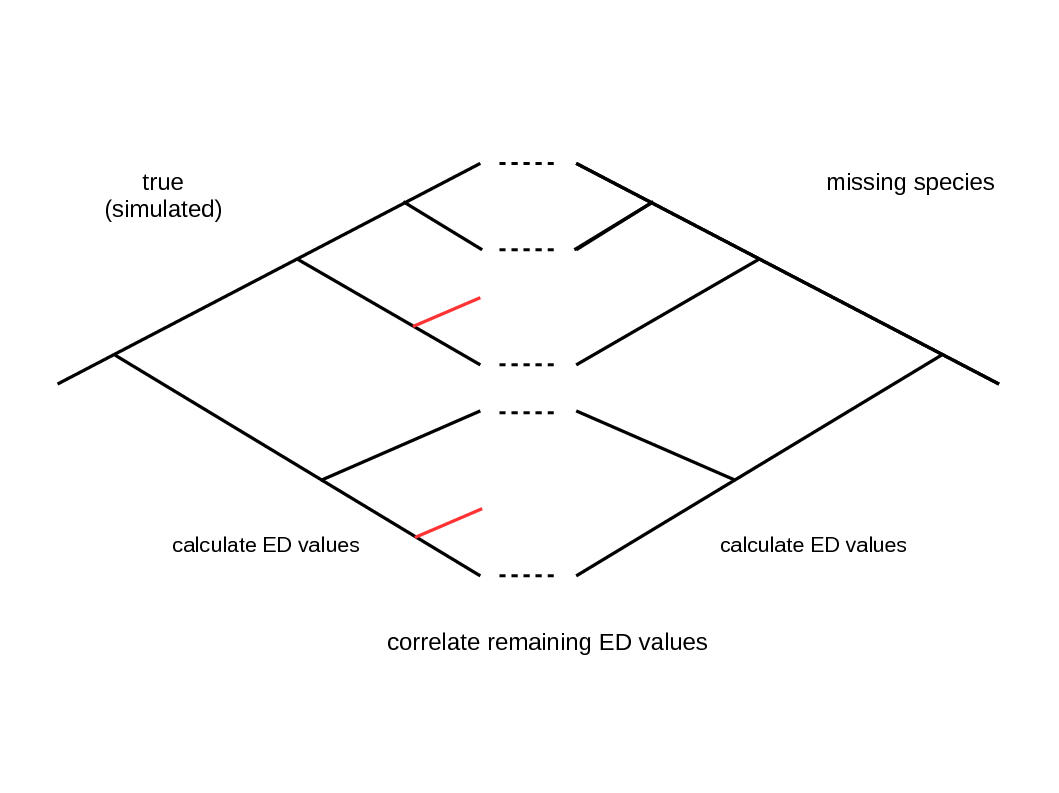
\includegraphics[width=.75\textwidth]{../figures/missingSpecies.png}
  \caption{\textbf{Conceptual overview of the missing-species simulations in
  this study.} The simulated tree on the left is the true tree prior to removal
  of missing species. On the right is the same tree after missing species have
  been removed. Species that are removed are shown in red. To compare the ED
  values of the remaining species, we correlate their ED values before (left)
  and after (right) removal of the missing species. Dashed lines can be seen for
  the species which would have ED scores compared.}
  \label{missingSpecies}
\end{figure}

\begin{figure}[!ht]
  \center
  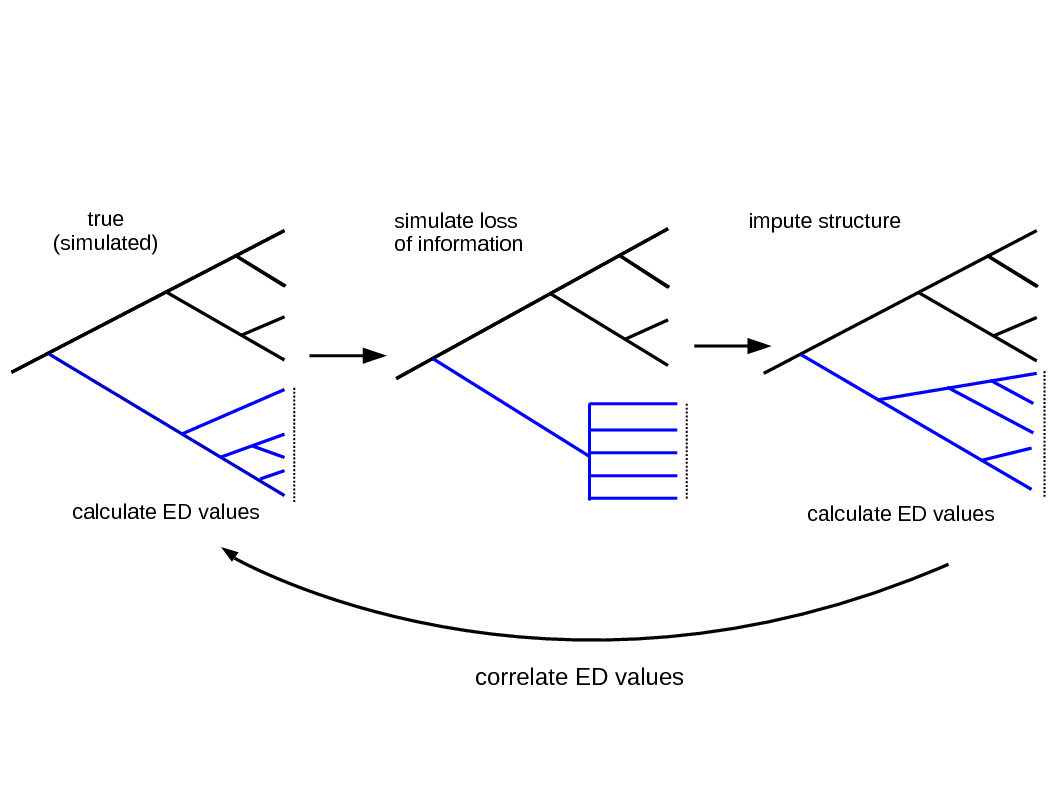
\includegraphics[width=.75\textwidth]{../figures/imputeConcept.png}
  \caption{\textbf{Conceptual overview of the imputation simulations conducted
  in this study.} The simulated tree on the left is the ‘true tree'. We selected
  a clade to treat as ‘missing' (highlighted with a dashed line and in blue) by
  treating it as a polytomy (middle panel), and then imputed the ‘missing'
  species to produce the imputed clade in the right panel. To compare true and
  imputed ED values within the imputed clade, we correlated ED values calculated
  for the true clade (left) with those for the imputed clade (right).}
  \label{imputeConcept}
\end{figure}

\begin{figure}[!ht]
  \center
  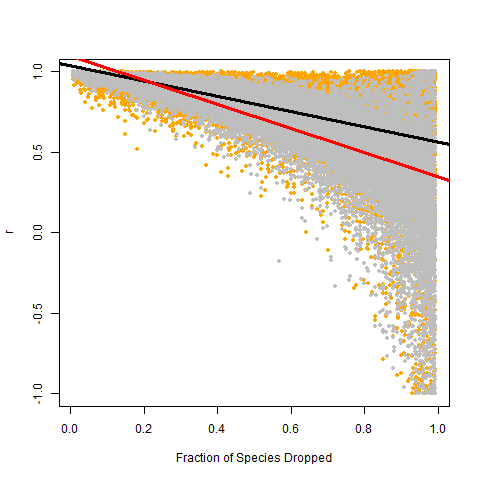
\includegraphics[width=.5\textwidth]{../figures/randomVsCluster.png}
  \caption{\textbf{The effect of missing data on the calculation of the
      remaining species' ED values.} The correlation coefficient of species' ED
      values in full (simulated) phylogenies, comparing values before and after
      the random loss of (other) species from the tree. The color of data points
      denote whether the species were removed from the phylogeny completely at
      random (orange) or in a phylogenetically biased fashion (see text; grey).
      Lines show regressions for random (red) or phylogenetically biased (black)
      species loss; see table \ref{missing_regression} for model coefficients.
      This plot shows that the accuracy of estimation of ED values is inversely
      proportional to the number of species missing from the phylogeny, and that
      phylogenetically-biased species loss has a greater impact on accuracy.}
  \label{randomVsClustered}
\end{figure}

\begin{figure}[!ht]
  \center
  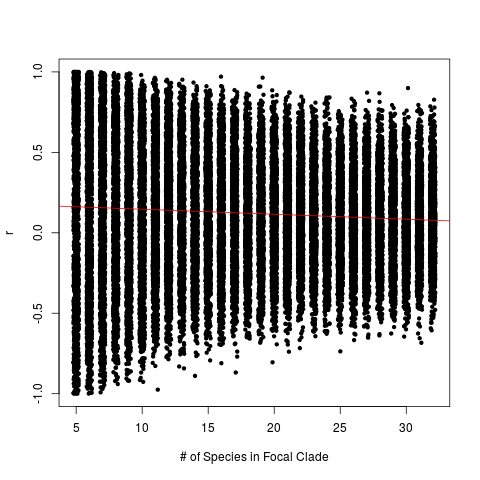
\includegraphics[width=.5\textwidth]{../figures/edModel.png}
  \caption{\textbf{The correlation between species' imputed and true ED scores
      plotted as a function of the number of species imputed (focal clade size
      from all sizes of phylogenies used (n = 128, ..., 1024)).} Each data point
      represents the correlation between ED values within the focal clades where
      imputation has occurred, comparing species' true ED values with their
      imputed ED values. This plot, and the statistical analysis of it in table
      \ref{impute_reg}, show limited support for an association between true and
      imputed ED values.}
  \label{imputationTrend}
\end{figure}

\begin{figure}[!ht]
  \center
  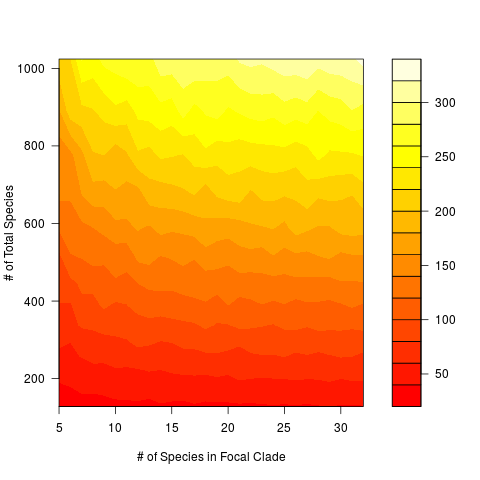
\includegraphics[width=.5\textwidth]{../figures/rankingError.png}
  \caption{\textbf{Mean ranking error of imputed species.} An
    interpolated heat-map of the mean ranking error of imputed species
    as a function of the total number of species in the phylogeny
    (vertical axis) and number of species in the focal (imputed) clade
    (horizontal axis). Table \ref{impute_rank} gives statistical
    support for the trend of increased error in larger phylogenies and
    imputed clades.\added{ This figure shows a tendency for an increase in error in larger phylogenies and imputed clades.}}
  \label{rankingError}
\end{figure}

\end{document}
%%% Local Variables:
%%% mode: latex
%%% TeX-master: t
%%% End:
